% !TEX root = ./main.tex
% !TEX encoding = UTF-8 Unicode
% !TEX program = pdflatex
% !TeX spellcheck = it_IT

\graphicspath{{Immagini/},{Immagini/dependability/}}

\chapter{Esercizi Dependability}
\section{Esercizio 1}
\subsection{Traccia}
\textit{Find the R(t) and MMTF for the system whose reliability diagram is given
below. In calculating. MTTF, assume all components are identical and fail
randomly with failure rate $\lambda$.}

\begin{figure}[!htbp]
  \centering
  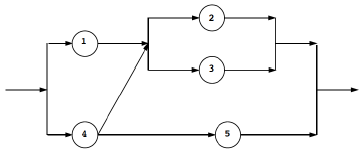
\includegraphics[width=\linewidth]{esercizio1}
  % \caption{}
  % \label{}
\end{figure}

\clearpage
\subsection{Soluzione}
In presenza di un \textit{Non-Series-Parallel-Systems} è possibile esplorare due
differenti approcci risolutivi:
\begin{itemize}
  \item \textbf{Teorema dell'\textit{Upper Bound}}: utilizzando la seguente formula è
  possibile stimare un upper bound della reliability del sistema.\\
  $$R_{sys} \leq 1-\prod_{i} f(i)$$
  In pratica, la tecnica prevede di considerare il parallelo tra tutti i possibili
  \textbf{success path} e calcolarne la reliability.\\
  Il risultato ottenuto è un upper bound della reliability effettiva del sistema.\\

  \item \textbf{Tecnica dell'espansione attorno ad un singolo nodo}: scegliendo
  un nodo del block diagram, è possibile studiare due casistiche:
  \begin{itemize}
    \item \textbf{Nodo Funzionante} - il nodo è sostituito con un circuito chiuso;
    \item \textbf{Nodo Fallente} - il nodo è sostituito con un circuito aperto.
  \end{itemize}
  In questo modo si studiano due sottosistemi effettivamente serie/parallelo,
  oppure, in caso contrario, si itera nuovamente il procedimento.\\
  Dopo aver calcolato la reliability dei due sottosistemi indipendentemente,
  applicando la \textit{Formula di Bayes}, si ottiene la reliability del sistema
  totale.\\
  $$R_{sys} = R_m \cdot P(system\ works \mid m\ works) + (1-R_m)\cdot P(system\ works \mid m\ fails)$$
\end{itemize}

\clearpage

\subsubsection{Caso 1 - Upper Bound}
In figura \ref{upperbound} è riportato il block diagram dei success path.

\begin{figure}[!htbp]
  \centering
  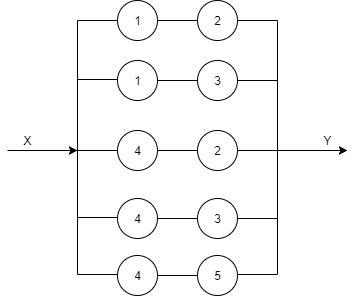
\includegraphics[width=.55\linewidth]{upperbound}
  \caption{Success Path}
  \label{upperbound}
\end{figure}

Calcolando la reliability del parallelo:
$$R_{sys} = 1-(1-R_1R_2) \cdot (1-R_1R_3) \cdot (1-R_4R_2) \cdot (1-R_4R_3) \cdot (1-R_4R_5)$$
Supponendo che ogni nodo ha stessa reliability: $$R_i = R$$
Si ottiene: $$R_{sys} = 1-(1-R^2)^5$$

\clearpage

\subsubsection{Caso 2 - Espansione del Nodo 4}
La Reliability del sistema, supponendo di espandere il nodo 4, sarà calcolata
utilizzando la seguente formula:
$$R_{sys} = R_4 \cdot P(system\ works \mid 4\ works) + (1-R_4)\cdot P(system\ works \mid 4\ fails)$$
ovvero:
$$R_{sys} = R_4 \cdot R_{4\ WORKS} + (1-R_4)\cdot R_{4\ FAILS}$$
dove $R_{4\ WORKS}$ e $R_{4\ FAILS}$ sono le reliability dei due sottosistemi,
definiti e studiati di seguito.\\
\subsubsection*{Nodo 4 Funzionante (works!)}
Nel caso in cui il nodo 4 funzioni, è possibile osservare che si creano
due differenti percorsi, nel sistema, per giungere al parallelo tra i nodi 2 e 3.\\
Un primo percorso attraverso il nodo 1, ed un secondo percorso diretto.\\
La presenza di un percorso diretto rende il calcolo della reliability del
sottosistema totalmente trasparente alla presenza del nodo 1.\\
Quindi, come mostrato in figura \ref{nodo1_eliminato}, il nodo 1 può non essere
considerato.\\
\begin{figure}[!htbp]
  \centering
  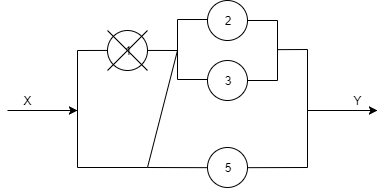
\includegraphics[width=.7\linewidth]{nodo1_eliminato}
  \caption{Eliminazione Nodo 1 a causa del percorso diretto}
  \label{nodo1_eliminato}
\end{figure}

\clearpage

\begin{figure}[!htbp]
  \centering
  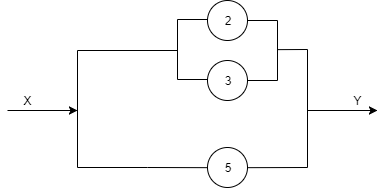
\includegraphics[width=.7\linewidth]{nodo4_funzionante}
  \caption{Sottosistema Risultante - Nodo 4 Funzionante}
  \label{nodo4_funzionante}
\end{figure}

Calcolo di $R_{4\ WORKS}$:
$$R_{4\ WORKS} = 1-(1-R_5)\cdot(1-R_{23})$$
dove:
$$R_{23} = 1-(1-R_2)\cdot(1-R_3)$$

Supponendo che tutti i nodo abbiano stessa reliability \textbf{R}, si ottiene:
$$R_{23} = 1-(1-R)^2$$
$$R_{4\ WORKS} = 1-(1-R)\cdot(1-R_{23})$$

\clearpage

\subsubsection*{Nodo 4 Fallente (not works!)}

\begin{figure}[!htbp]
  \centering
  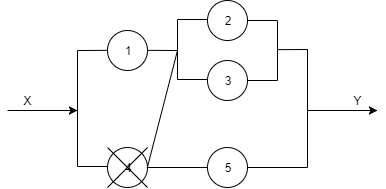
\includegraphics[width=.7\linewidth]{nodo4_eliminato}
  \caption{Eliminazione Nodo 4}
  \label{nodo4_eliminato}
\end{figure}

L'eliminazione del nodo 4 crea una spaccatura nel sistema, rendendo il nodo 5
irraggiungibile.\\

\begin{figure}[!htbp]
  \centering
  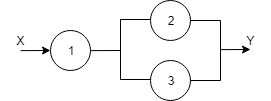
\includegraphics[width=.6\linewidth]{nodo4_fallente}
  \caption{Sottosistema Risultante - Nodo 4 Fallente}
  \label{nodo4_fallente}
\end{figure}

Calcolo di $R_{4\ FAILS}$:
$$R_{4\ FAILS} = R_1 \cdot R_{23} = R_1 \cdot (1-(1-R_2)\cdot(1-R_3))$$

Supponendo che tutti i nodo abbiano stessa reliability \textbf{R}, si ottiene:
$$R_{4\ FAILS} = R \cdot (1-(1-R)^2)$$

\clearpage

\subsubsection{Calcolo $R_{sys}$ del sistema}
Dopo aver calcolato separatamente $R_{4\ WORKS}$ e $R_{4\ FAILS}$, è possibile
proseguire con il calcolo della reliability totale del sistema, supponendo che
tutti i nodo abbiano stessa reliability \textbf{R}:
$$R_{sys} = R \cdot R_{4\ WORKS} + (1-R)\cdot R_{4\ FAILS} =$$
$$= R(1-(1-R)(1-1+(1-R)^2)) + R(1-R)(1-(1-R)^2) =$$
$$= 5R^2-6R^3+2R^4$$

Per quanto riguarda il \textbf{MTTF}, in seguito sono riportati
i calcoli dell'integrale:
$$R(t) = e^{-\lambda t}$$
$$\int_0^{+\infty} R_{sys}(t)\ dx =
\int_0^{+\infty} (5e^{-2\lambda t}-6e^{-3\lambda t}+2e^{-4\lambda t}) \ dx =
\frac{5}{2\lambda} - \frac{2}{\lambda} + \frac{1}{2\lambda} =
\frac{1}{\lambda}$$

\clearpage

\section{Esercizio 2}
\subsection{Traccia}
\textit{We want to compare two different schemes of increasing reliability of a
system using redundancy. Suppose that the system needs s identical components
in series for proper operation. Further suppose that we are given (m x s)
components. Out of the two schemes shown in the figure below, which one will
provide a higher reliability? Given that the reliability of an individual
component is r, derive the expressions for the reliabilities of two configurations.
For m = 5 and s = 2, compare the two expressions.}

\begin{figure}[!htbp]
  \centering
  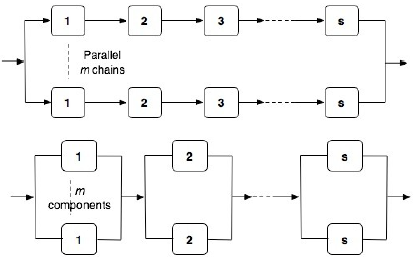
\includegraphics[width=\linewidth]{esercizio2}
  % \caption{}
  % \label{}
\end{figure}

\clearpage
\subsection{Soluzione}

\subsubsection{Schema A}

\begin{figure}[!htbp]
  \centering
  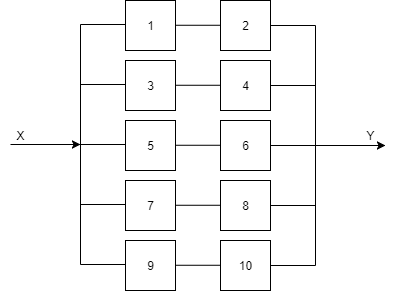
\includegraphics[width=.7\linewidth]{parallelo_serie}
  \caption{Paralleli di Serie}
  \label{parallelo_serie}
\end{figure}

Nel primo schema riportato in figura \ref{parallelo_serie} si osserva una
struttura composta da 5 paralleli, ciascuno di 2 nodi posti in serie.\\
La reliability totale del sistema, in questo caso, si calcola facilmente:
$$R_{sys\ A} = 1-(1-R_1R_2)\cdot(1-R_3R_4)\cdot(1-R_5R_6)\cdot(1-R_7R_8)\cdot(1-R_9R_{10})$$
supponendo identiche le reliability di ciascun nodo:
\begin{align}
  R_{sys\ A} = 1-(1-R^2)^5
 \label{eq1}
\end{align}
Ricordando che da specifica erano $s=2$ e $m=5$, è possibile generalizzare la
formula come segue:
$$R_{sys\ A} = 1-(1-R^s)^m$$

\clearpage

\subsubsection{Schema B}

\begin{figure}[!htbp]
  \centering
  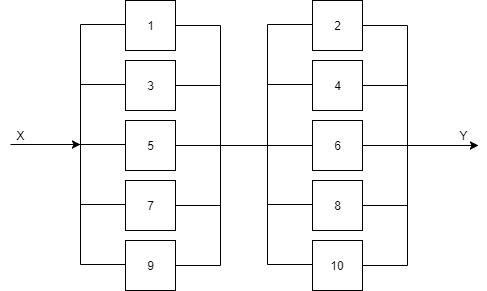
\includegraphics[width=.7\linewidth]{serie_parallelo}
  \caption{Serie di Paralleli}
  \label{serie_parallelo}
\end{figure}

Nel secondo schema riportato in figura \ref{serie_parallelo} si osserva una
struttura composta da 5 serie, ciascuna di 2 nodi posti in parallelo.\\
La reliability totale del sistema, in questo caso, si calcola facilmente:
$$R_{sys\ B} = [1-(1-R_1)(1-R_3)(1-R_5)(1-R_7)(1-R_9)]\cdot[1-(1-R_2)(1-R_4)(1-R_6)(1-R_8)(1-R_{10})]$$
supponendo identiche le reliability di ciascun nodo:
\begin{align}
  R_{sys\ B} = [1-(1-R)^5]^2
 \label{eq2}
\end{align}
Ricordando che da specifica erano $s=2$ e $m=5$, è possibile generalizzare la
formula come segue:
$$R_{sys\ B} = [1-(1-R)^m]^s$$

\clearpage

\subsubsection{Confronto $R_{sys}$ dei due schemi}
Per confrontare le reliability nei due casi, conviene espandere le espressioni
calcolate in  \eqref{eq1} e \eqref{eq2}.
$$R_{sys\ A} = 1-(1-R^2)^5 = 5R^2-10R^4+10R^6-5R^8+R^{10}$$
$$R_{sys\ B} = [1-(1-R)^5]^2 = 25R^2-100R^3+200R^4-250R^5+210R^6-120R^7+45R^8-10R^9+R^{10}$$
\vspace{0.3cm}

Supponendo $R_{sys\ B} > R_{sys\ A}$ e semplificando la disequazione, si ottiene:
$$R^3<R^2 \ \ \ \ per \ 0<R<1$$
Quest'assunzione è sempre vera, essendo la reliability una probabilità.\\
Quindi è possibile concludere che la reliability del sistema B è sempre
maggiore a quella del sistema A, come mostrato anche dal plot in figura \ref{confronto_reliability}.\\

\begin{figure}[!htbp]
  \centering
  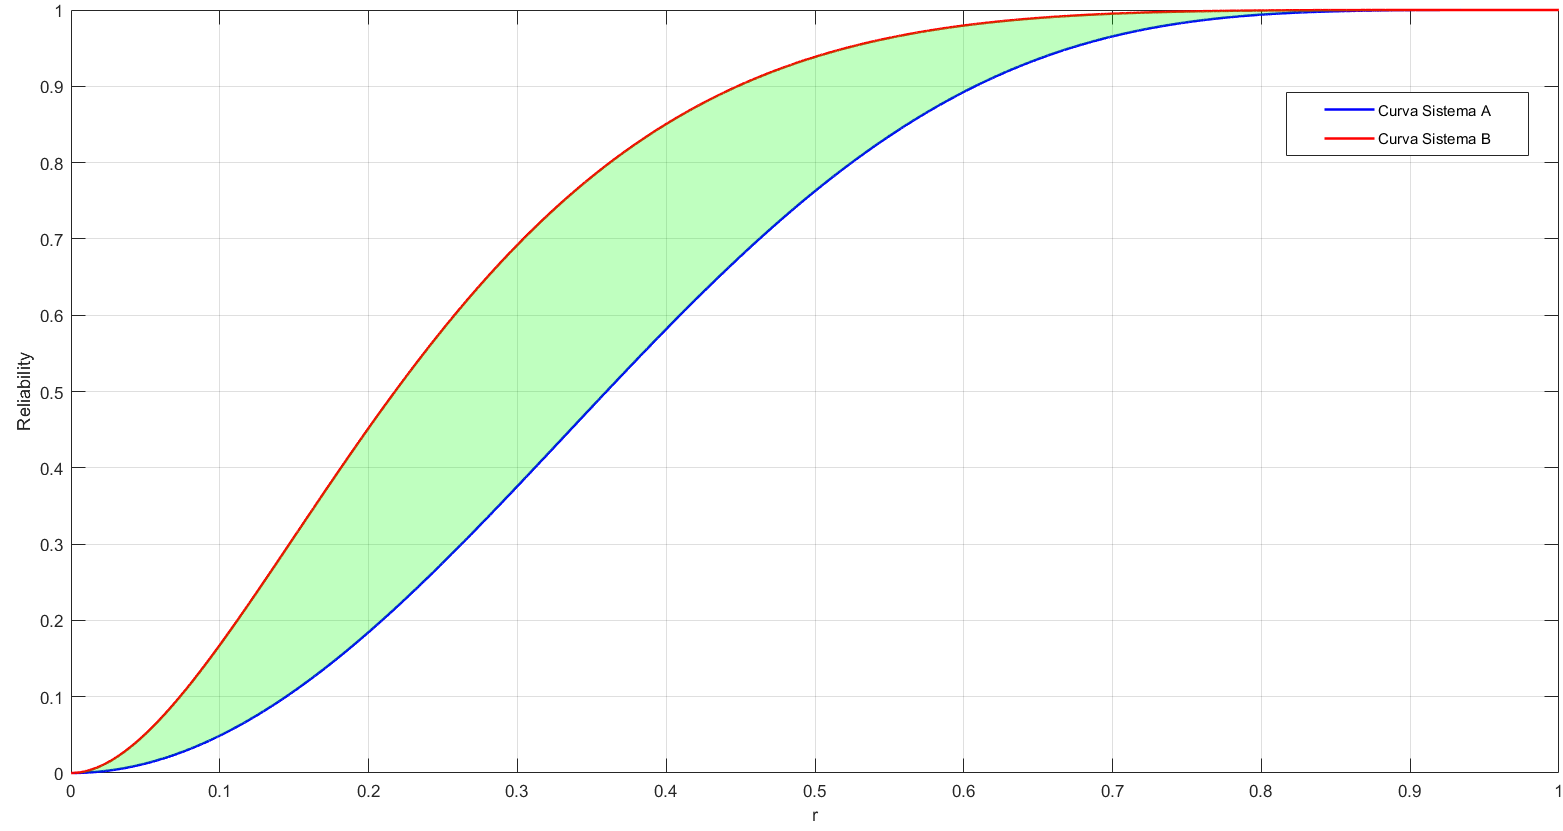
\includegraphics[width=\linewidth]{confronto_reliability}
  \caption{Plot Reliability Sistema A Vs Sistema B}
  \label{confronto_reliability}
\end{figure}

\clearpage

\section{Esercizio 3}
\subsection{Traccia}
\textit{The architecture of a network of computers in a banking system is shown
below. The architecture is called a skip-ring network and is designed to allow
processors to communicate even after node failures have occurred. For example,
if node 1 fails, node 8 can bypass the failed node by routing data over the
alternative link connecting nodes 8 and 2. Assuming the links are perfect and
the nodes each have a reliability of Rm, derive and expression for the reliability
of the network. If Rm obeys the exponential failure law and the failure rate of
each node is 0.005 failures per hour, determine the reliability of the system
at the end of a 48-hour period.}
\begin{figure}[!htbp]
  \centering
  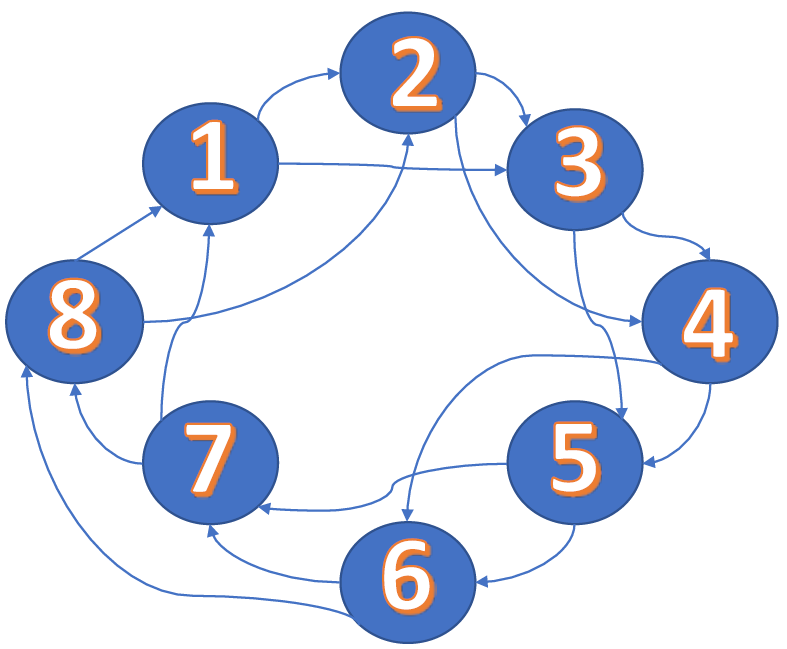
\includegraphics[width=.7\linewidth]{esercizio3}
  % \caption{}
  % \label{}
\end{figure}

\clearpage
\subsection{Soluzione}

La rete presentata è in grado di funzionare fino ad un massimo di 4 nodi fallimentari
e può essere ricondotta ad un modello \textbf{M-out-of-N Systems}, con M uguale 4
ed N uguale 8.\\
Dunque la reliability è data dalla seguente espressione:
$$ R = \sum_{i=0}^{4}{\binom{8}{i}R_m^{8-i}(1-R_m)^i}$$

Osservando che per:
\begin{itemize}
  \item \textbf{\textit{i=0}}: il sistema non fallisce;
  \item \textbf{\textit{i=1}}: il sistema non fallisce poiché la condizione necessaria
  per il fallimento è che falliscano due nodi consecutivi;
  \item \textbf{\textit{i=2}}: il sistema fallisce solo in 8 casi, quindi
  nella formula va utilizzato il coefficiente binomiale meno le 8 combinazioni che
  portano il sistema al fallimento;
  \item \textbf{\textit{i=3}}: il sistema fallisce in 40 casi, 8 combinazioni di 3 nodi consecutivi, 32 combinazioni
  di 2 nodi consecutivi + 1 nodo non adiacente;
  \item \textbf{\textit{i=4}}: il sistema non fallisce solo in due casi ovvero
  (1, 3, 5, 7) e (2, 4, 6, 8);
  \item \textbf{\textit{i=5, i=6, i=7}}: il sistema fallisce sempre, poiché
  falliscono sempre almeno due nodi consecutivi;
  \item \textbf{\textit{i=8}}: il sistema fallisce poiché tutti i nodi falliscono.
\end{itemize}

\begin{tabular}{c||c|c|}

\textbf{Nodi falliti}& \textbf{P(nodi falliti)} & \textbf{P(fallimento sistema $\mid$ n nodi falliti)}\\
\hline
\hline
0 & $r^8$ & 0 \\
\hline
1 & $8(1-r)r^7$ & 0 \\
\hline
2 & $28(1-r)^2r^6$ & $8/28$ \\
\hline
3 & $56(1-r)^3r^5$ & $40/56$ \\
\hline
4 & $70(1-r)^4r^4$ & $68/70$ \\
\hline
5 & $56(1-r)^5r^3$ & $1$ \\
\hline
6 & $28(1-r)^6r^2$ & $1$ \\
\hline
7 & $8(1-r)^7r$ & $1$ \\
\hline
8 & $(1-r)^8$ & $1$ \\
\hline
\end{tabular}

\clearpage

Considerando $R_m=e^{-\lambda t}=e^{-0,005\cdot 48}=0,786627861$ si ottiene:
$$R=R_m^8+8R_m^7(1-R_m)+(28-8)R_m^6(1-R_m)^2+(56-40)R_m^5(1-R_m)^3+(70-68)R_m^4(1-R_m)^4$$
$$R=0,728880175$$

\clearpage
\section{Esercizio 4}
\subsection{Traccia}
\textit{An application requires that at least three processors from a multiprocessor
system be available with more than 99\% probability. The cost of a processor with
80\% reliability is \$1000, and each 10\% increase in reliability will cost \$800.
Determine the number of processors (n) and the reliability (p) of each processor
(assume that all processors have the same reliability) that minimize the total
system cost.}

\clearpage
\subsection{Soluzione}
Il sistema proposto nella traccia è un tipico \textbf{M-out-of-N System}.\\
In questo caso particolare, il numero minimo di processori richiesto è 3, quindi
il modello diventa un 3-out-of-N System.\\
La reliability di tale sistema si calcola semplicemente applicando la seguente
formula:
$$R_{sys} = \sum_{i=0}^{N-3} \binom{N}{i} R_m^{N-i}(1-R_m)^i$$
\vspace{0.4cm}

Il costo del singolo processore dipende dalla reliability che si desidera ottenere.\\
Un processore con 80\% di reliability costa \$1000, ogni incremento del 10\% di
reliability ha un costo di \$800 sul totale.\\
\'E stato scelto di analizzare due differenti casi:
\begin{itemize}
  \item Processore con Reliability 80\% - Costo \$1000
  \item Processore con Reliability 90\% - Costo \$1800
\end{itemize}

\clearpage

In funzione di queste due soluzioni, sono state realizzate delle tabelle che
mostrano la reliability ottenuta al prezzo $C_i$, al variare del numero di processori
e della loro tipologia.\\

\begin{figure}[!htbp]
  \centering
  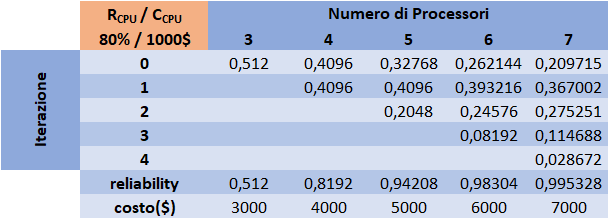
\includegraphics[width=\linewidth]{costo_processori_rel80}
  \caption{Sistema nel caso di utilizzo di Processori con 80\% reliability}
  \label{costo_processori_rel80}
\end{figure}

\begin{figure}[!htbp]
  \centering
  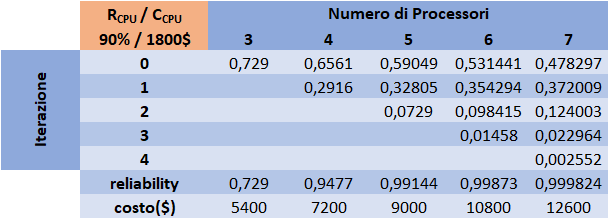
\includegraphics[width=\linewidth]{costo_processori_rel90}
  \caption{Sistema nel caso di utilizzo di Processori con 90\% reliability}
  \label{costo_processori_rel90}
\end{figure}

Osservando i risultati tabellati, la combinazione con reliability al 99\% con
costo minore risulta essere:
\begin{itemize}
  \item \textbf{N=7} processori da 80\% di reliability, costo \$7000;
  \item \textbf{N=5} processori da 90\% di reliability, costo \$9000.
\end{itemize}

\clearpage

\section{Esercizio 5}
\subsection{Traccia}
\textit{The system shown in the figure below is a processing system for a helicopter. The system
has dual-redundant processors and dual-redundant interface units. Two buses are used in
the system, and each bus is also dual-redundant. The interesting part of the system is the
navigation equipment. The aircraft can be completely navigated using the Inertial
Navigation System (INS). If the INS fails, the aircraft can be navigated using the
combination of the Doppler and the altitude heading and reference system (AHRS). The
system contains three AHRS units, of which only one is needed. This is an example of
functional redundancy where the data from the AHRS and the Doppler can be used to
replace the INS, if the INS fails. Because of the other sensors and instrumentation, both
buses are required for the system to function properly regardless of which navigation mode
is being employed.}

\begin{figure}[!htbp]
  \centering
  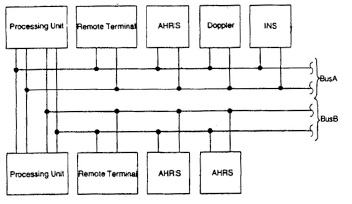
\includegraphics[width=.7\linewidth]{esercizio5}
  % \caption{}
  \label{esericizo5}
\end{figure}

\begin{enumerate}
  \item Draw the reliability block diagram of the system;
  \item Draw the Fault Tree of the system and analyze the minimal cutsets;
  \item Calculate the reliability for a one-hour flight using the MTTF figures given in the table
  below. Assume that the exponential failure low applies and that the fault coverage is perfect.

  \begin{center}
  \begin{tabular}{|c|c|}
  	\hline
  	\textbf{Equipment} & \textbf{MTTF(hr)} \\
  	\hline
  	Processing Unit  & 3000 \\
  	\hline
  	Remote Terminal  & 2500 \\
  	\hline
  	AHRS & 1000 \\
  	\hline
  	INS & 1000 \\
  	\hline
  	Doppler & 500 \\
  	\hline
  	Bus & 8000 \\
  	\hline
  \end{tabular}
  \end{center}

  \item Repeat (c), but this time, incorporate a coverage factor for the fault
  detection and reconfiguration of the processing units. Using the same failure
  data, determine the approximate fault coverage value that is required to obtain
  a reliability (at the end of one hour) of 0.99999.
\end{enumerate}

\clearpage
\subsection{Soluzione}

\subsection{Quesito a: Reliable Block Diagram}

Il \textbf{Reliable Block Diagram(RBD)} è uno strumento che permette di studiare
la reliability di un sistema in modo semplice, sfruttandone lo schema a blocchi.\\

\begin{figure}[!htbp]
  \centering
  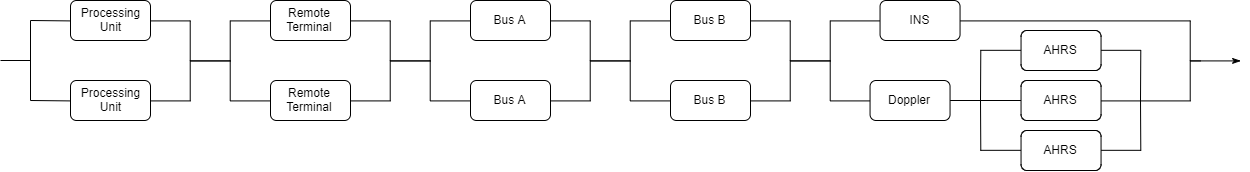
\includegraphics[width=\linewidth]{rdb}
  \caption{Reliable Block Diagram(RBD)}
  \label{rdb}
\end{figure}

I componenti \textit{CPU}, \textit{Remote Terminal}, \textit{Bus(A e B)} sono
dual-redundant, quindi sono duplicati e messi in parallelo, mentre \textit{INS} è
in parallelo con la serie tra \textit{Doppler} e il parallelo dei tre \textit{AHRS}.\\
Infine i cinque sottosistemi sono in serie.

\subsection{Quesito b: Fault Tree and minimal cut-set}

Il \textbf{Fault Tree} è uno strumento che permette di individuare i componenti
causanti il fallimento del sistema fallisce, da esso si può ricavare il minimo numero di
componenti che porta il sistema al fallimento.

\begin{figure}[!htbp]
  \centering
  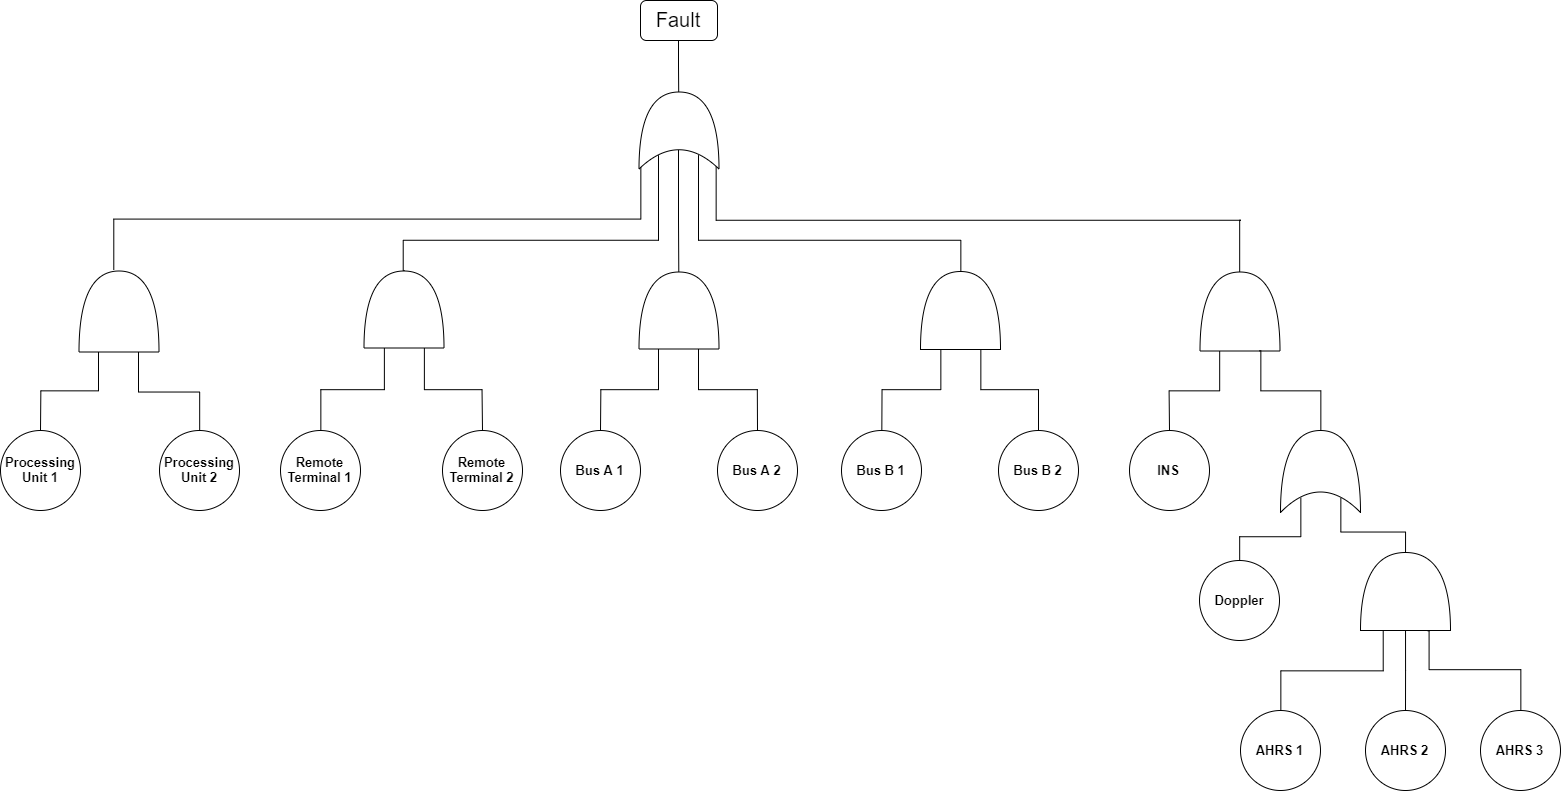
\includegraphics[width=\linewidth]{ft}
  \caption{Fault Tree}
  \label{ft}
\end{figure}

Il fault tree può essere ricavato a partire da un RBD, trasformando
la serie di due componenti in una \textit{OR} ed il parallelo in una \textit{AND}.\\

\'E possibile scrivere in forma analitica il fault tree riportato in \figurename~\ref{ft}:
$$ F = (PU_1 \cdot PU_2) + (RT_1 \cdot RT_2) + (BUS_{A1} \cdot BUS_{A2}) + (BUS_{B1} \cdot BUS_{B2})+$$
$$+ (INS \cdot (Doppler+AHRS_1 \cdot AHRS_2 \cdot AHRS_3))$$

Può essere riscritta in funzione dei mintermini:
$$ F = (PU_1 \cdot PU_2) + (RT_1 \cdot RT_2) + (BUS_{A1} \cdot BUS_{A2}) + (BUS_{B1} \cdot BUS_{B2})+$$
$$+ (INS \cdot Doppler) + (INS \cdot AHRS_1 \cdot AHRS_2 \cdot AHRS_3)$$

\clearpage

\subsection{Quesito c: Reliability for one-hour flight}

Supponendo che la distribuzione dei fallimenti sia esponenziale, si ha che la
Reliability dell'i-esimo componente è:
$$R_i(t) = e^{-\lambda_i t}$$

Per il calcolo di $\lambda_i$, conoscendo la \textbf{\textit{MTTF}}, si utilizza
la relazione:
$$ MTTF = \int_{0}^{+\infty} e^{-\lambda t}\, dt = \frac{1}{\lambda} \ \ \Longrightarrow \ \ \lambda = \frac{1}{MTTF} $$

In \figurename~\ref{reliability_es5} sono riportate le reliability per un'ora di
volo per ogni componente.\\

\begin{figure}[!htbp]
  \centering
  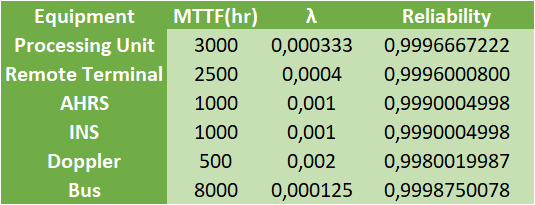
\includegraphics[width=0.6\linewidth]{reliability_es5}
  \caption{Reliability di ogni componente in un'ora di volo}
  \label{reliability_es5}
\end{figure}

Considerando la \figurename~\ref{rdb} si applicano le formule per il calcolo
della reliability per componenti in serie e parallelo.\\
In particolare:
\begin{itemize}
  \item \textbf{Reliability di una serie} $\rightarrow R_{serie} = \prod_{i=1}^{N}{R_i(t)}$;
  \item \textbf{Reliability di una serie} $\rightarrow R_{parallelo} = 1 - \prod_{i=1}^{N}{(1- R_i(t))}$.
\end{itemize}

Dunque la reliability del sistema è calcolata come:
$$ R_{sys} = R_{subSys_1} \cdot R_{subSys_2} \cdot R_{subSys_3} \cdot R_{subSys_4} \cdot R_{subSys_5}$$
dove:
$$R_{subSys_1} = 1 - (1 - R_{ProcessingUnit})^2$$
$$R_{subSys_2} = 1 - (1 - R_{RemoteTerminal})^2$$
$$R_{subSys_3} = 1 - (1 - R_{BusA})^2$$
$$R_{subSys_4} = 1 - (1 - R_{BusB})^2$$
$$R_{subSys_5} = 1 - (1 - R_{INS}) \cdot (1 - R_{subSys_{51}})$$
$$R_{subSys_{51}} = R_{Doppler} \cdot (1 - (1 - R_{AHRS})^3)$$

\clearpage

In \figurename~\ref{calcolo_rel} sono riportati i risultati parziali e la
reliability del sistema.\\

\begin{figure}[!htbp]
  \centering
  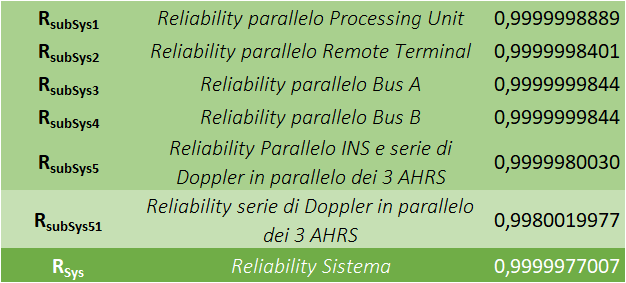
\includegraphics[width=0.6\linewidth]{calcolo_rel}
  \caption{Calcolo Reliability in un'ora di volo}
  \label{calcolo_rel}
\end{figure}

Quindi dopo un'ora di volo la reliability dell'intero sistema è 99,99977007\%.\\

\clearpage

\subsection{Quesito c: Reliability one-hour flight with coverage}

Per calcolare il fattore di coverage per la fault detection e per la riconfigurazione
della Processing Unit, al fine di ottenere una reliability di 5 nine, sarà ripetuto
il procedimento del quesito precedente introducendo un fattore di coverage(c).\\
Dunque:
$$R_{subSys_1} = 1 -[ (1 - R_{ProcessingUnit}) \cdot (1-c\cdot R_{ProcessingUnit})]$$
$$R_{subSys_2} = 1 - (1 - R_{RemoteTerminal})^2$$
$$R_{subSys_3} = 1 - (1 - R_{BusA})^2$$
$$R_{subSys_4} = 1 - (1 - R_{BusB})^2$$
$$R_{subSys_5} = 1 - (1 - R_{INS}) \cdot (1 - R_{subSys_{51}})$$
$$R_{subSys_{51}} = R_{Doppler} \cdot (1 - (1 - R_{AHRS})^3)$$
Per calcolare $c$ si ha:
$$R_{subSys_1} = R_{ProcessingUnit}+c\cdot(1-R_{ProcessingUnit} )\cdot R_{ProcessingUnit}$$
$$R_{Sys-ProcessingUnit} =  R_{subSys_2} \cdot R_{subSys_3} \cdot R_{subSys_4} \cdot R_{subSys_5}$$
$$R_{Sys}=[R_{ProcessingUnit}+c\cdot(1-R_{ProcessingUnit})\cdot R_{ProcessingUnit}]\cdot R_{Sys-ProcessingUnit}$$

\vspace{0.4cm}
Volendo ottenere la reliability del sistema di 5 nine si impone $R_{Sys}=0,99999$.\\
Dunque si ottiene:
$$[R_{ProcessingUnit}+c\cdot(1-R_{ProcessingUnit})\cdot R_{ProcessingUnit}]\cdot R_{Sys-ProcessingUnit}=0,99999$$
Quindi:
$$ c = \frac{0,99999-R_{ProcessingUnit}\cdot R_{Sys-ProcessingUnit}}{(1-R_{ProcessingUnit})\cdot R_{ProcessingUnit} \cdot R_{Sys-ProcessingUnit}}$$

\vspace{0.4cm}
Sostituendo con i valori calcolati nel quesito precedente $c=0,97688$.\\
